\documentclass[10pt]{article}
\usepackage[left=0.9in,top=0.9in,bottom=0.9in,right=0.9in]{geometry}
\usepackage{setspace}
\usepackage{titlesec}
\usepackage{graphicx}
\usepackage{float}
\usepackage{mathtools}
\usepackage{amsmath}
\usepackage[font=small,labelfont=bf,labelsep=period]{caption}
\usepackage[english]{babel}
\usepackage{indentfirst}
\usepackage{array}
\usepackage{makecell}
\usepackage[usenames,dvipsnames]{xcolor}
\usepackage{multirow}
\usepackage{tabularx}
\usepackage{arydshln}
\usepackage{caption}
\usepackage{subcaption}
\usepackage{xfrac}
\usepackage[numbers,sort&compress]{natbib}
\usepackage{enumitem}
\usepackage{lipsum}
\usepackage{hyperref}
\usepackage{caption}
\setlength{\bibsep}{0pt}

%\usepackage{setspace}
%\onehalfspacing
\linespread{1.3}  % one-half spacing

%\pagestyle{fancy} 
%\fancyhead[LE,RO]{\today}
%\fancyhead[C]{NE 255}
%\fancyhead[LO,RE]{D. Hellfeld}
%\fancyfoot[C]{\thepage\ of \pageref{LastPage}}
%\renewcommand{\headrulewidth}{0.4pt}
%\renewcommand{\footrulewidth}{0.4pt}

\pagestyle{empty}

% Set up figure/table captions
\addto\captionsenglish{\renewcommand{\figurename}{Fig.}}
\addto\captionsenglish{\renewcommand{\tablename}{\small Table}}
\renewcommand{\thetable}{\Roman{table}}
\captionsetup[table]{labelfont = normal, labelsep=period, singlelinecheck=false}
\captionsetup[figure]{labelfont=normal, labelsep=period, singlelinecheck=true}

%\setlength\parindent{0pt}

% Set up section\subsection title formats
\renewcommand{\thesection}{\Roman{section}}
\renewcommand{\thesubsection}{\thesection.\Roman{subsection}}
\titleformat*{\section}{\normalsize\bfseries}
\titleformat*{\subsection}{\normalsize\bfseries}

\begin{document}

\begin{centering}
\textbf{Monte Carlo Simulation and Analysis Framework for a CdZnTe-based Spherical Coded\\[-5pt] Aperture and Compton Gamma-ray Imager}\\
\vspace{5pt}
NE 255 - Numerical Simulation in Radiation Transport \\[-5pt]
University of California, Berkeley \\[-5pt]
Department of Nuclear Engineering\\
\vspace{5pt}
Daniel Hellfeld\\
\vspace{5pt}
November 15, 2016 \\
\end{centering}


% -----------------------------------------------------------------------
\section{Introduction}

The goal of this project is to improve a Geant4 \cite{Agostinelli2003} Monte Carlo simulation for the Portable Radiation Imaging Spectroscopy and Mapping (PRISM) detector system under development at Lawrence Berkeley National Laboratory (LBNL) (see \hyperlink{fig1}{Fig.\,1a-b}) and to develop a small suite of analysis tools. The PRISM system consists of cm$^3$ CdZnTe (CZT) coplanar grid (CPG) gamma-ray detectors arranged on the inner surface of a 14 cm diameter sphere. There are 192 available detector locations on the sphere, but an active coded arrangement, or a pattern of occupied and empty locations (see \hyperlink{fig1}{Fig.\,1c}), of the detectors allows for gamma-ray imaging in 4$\pi$ using both coded aperture (low energy) and Compton imaging (high energy) modalities. The purpose of the simulation is to determine the response of the system to radioactive sources of varying energies, intensities, and spatial distributions in the entire 4$\pi$ field-of-view (FOV). The simulated response can then be used as a tool to inform prototype design, for characterization, and for image reconstruction. 

The original simulation was developed in order to generate a simple approximation of the coded aperture response in the far-field limit (parallel rays at infinity). The simulation essentially functioned as a ray-tracer (i.e. no scattering, no secondary electron tracking), however some physics was included to account for the depth-of-interaction (DOI) in each detector. This project aims to restructure and upgraded the original simulation to include more functionality such as scattering physics, secondary electron production and tracking, multi-site events, geometry modification, and near-field sources with varying strengths and distributions. In addition to the simulation, analysis tools used for event sequencing, data preprocessing, and 2D/3D image reconstruction will be developed. The ultimate objective of this project is to develop a high-fidelity, robust, flexible, well-documented, and easy to use simulation and analysis framework that can be used to answer a variety of research questions for the novel concept of a spherical coded aperture and Compton imaging system. 

%The first major step in completing this project is to filter the existing code and to establish a working baseline simulation. This will include setting up a version control repository (git) and transferring all the preexisting source and header files (written in C\texttt{++}) as well as restructuring the build scripts (CMake). Simple tests will be performed to ensure the base code is functional. This should be completed by 10/28/16. A thorough investigation into the physics lists available in Geant4 will be conducted and the necessary physics packages will be chosen by 10/31/16. This will include learning how exactly the libraries are modeling certain physics phenomenon and how sampling is done internally in Geant4. The geometry is currently hard-coded in the simulation and thus leaves little room for user adjustments. The geometry building code will be restructured to use formatted geometry files and messenger classes will be developed to allow the user to make in-simulation adjustments to the geometry (this will be very useful when running simulations to optimize the configuration of detectors). Various detector properties (i.e. tallies) currently exist for the geometry (such as time, energy, and position), but a messenger class will be developed to easily turn certain features on and off.  Some form of uncertainty quantification in the tallies will also need to be explored, which will require a literature review into how this is done in Geant4. All the geometry work should be completed by 11/4/16. Next, code will be written to enable flexible source particle generation. This will include far-field (parallel rays) sources, near-field sources (used for 3D imaging), point and extended sources, and a Poisson sampler to simulate a user defined source strength and acquisition time. This will require some thought into appropriate source biasing techniques in order to efficiently simulate particles without large computational costs. This should be completed by 11/11/16. Finally, a more efficient file writing architecture will be developed to quickly write compact output files. System response simulations can be quite large (many particles and many different source locations) therefore most output will need to be written in binary. This will require a more thorough understanding of the Geant4 framework to determine how to store data and when it is best to write data. This should be completed by 11/19/16. Finally, a suite of analysis tools will be developed to accompany the simulation output. This will include reading binary files, organization of data, preprocessing of data (such as event sequencing, coincidence detection, energy cutoffs, and time cutoffs), and image reconstruction for both coded aperture (back-projection, cross-correlation, and Maximum Likelihood Expectation Maximization (MLEM)) and Compton imaging (cone back-projection and MLEM) in 2D (and 3D, if term permits). This will require a literature review into coded aperture and Compton imaging methods and testing of several implementations. This should be completed by 12/2/16. In the final week, several test cases (for both near-field and far-field coded aperture and Compton imaging) will be simulated and analyzed. The results (as well as the work leading up to the results) will be documented into a final report and presented by 12/14/16.

\vspace{10pt}
\begin{figure}[htb]
\hypertarget{fig1}{}
\centering
\begin{tabular}{ccc}
	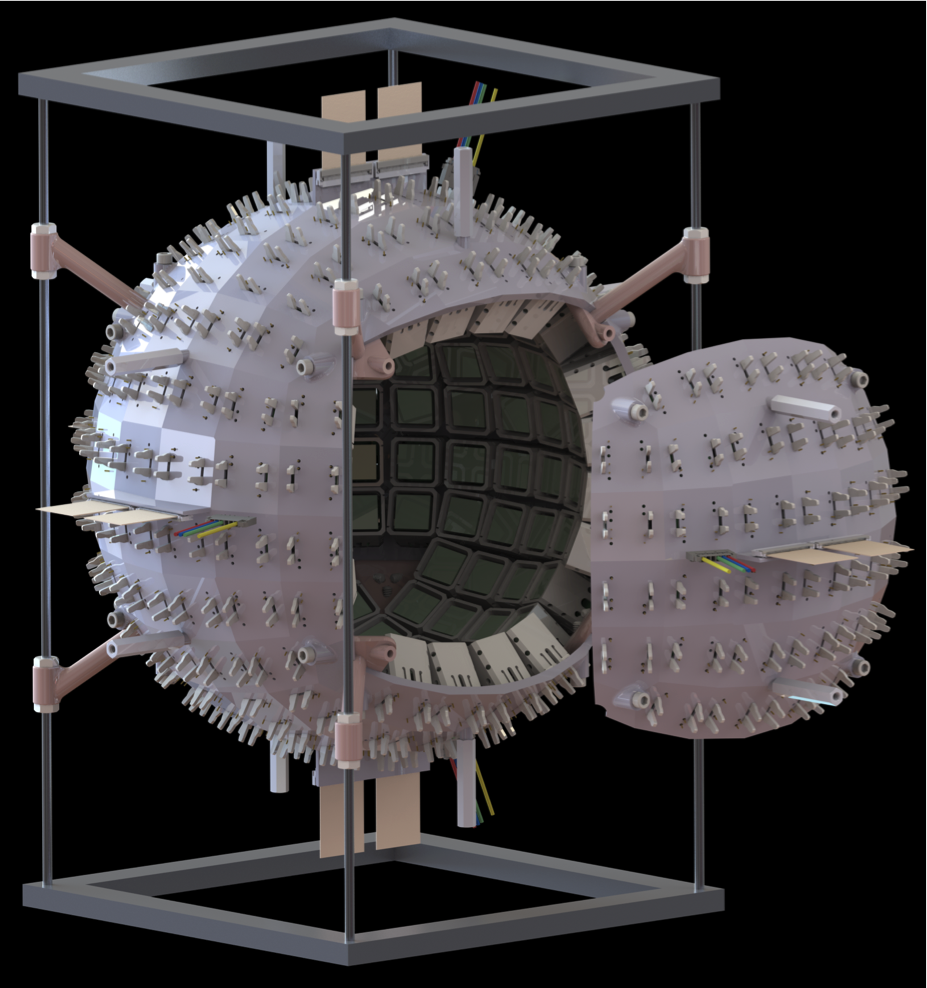
\includegraphics[height=130pt]{Figures/PRISM_Design.png} & 
	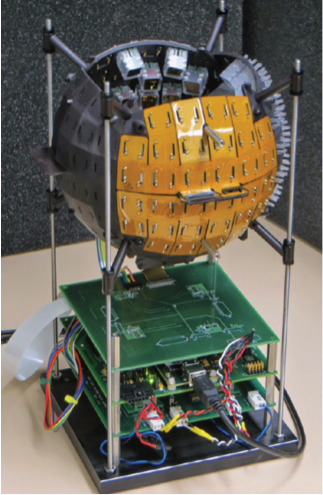
\includegraphics[height=130pt]{Figures/PRISM_Prototype.png} & 
	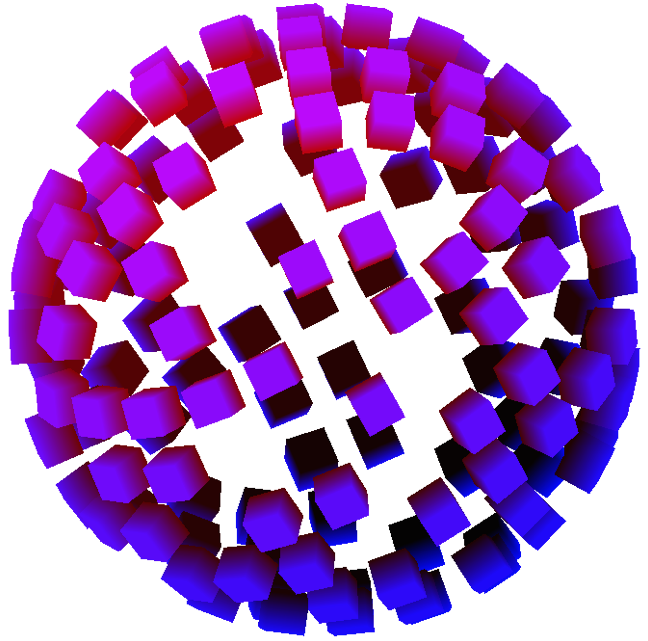
\includegraphics[height=130pt]{Figures/Masked_Configuration.png} \\
	\scriptsize{(a)} & \scriptsize{(b)} & \scriptsize{(c)} \\[-6pt]
\end{tabular}
\caption{(a) Modular design of PRISM. (b) PRISM prototype system currently under development at LBNL. (c) Example coded arrangement of detectors.}
\end{figure}


Outline the rest of the report here...



% -----------------------------------------------------------------------
\section{Mathematics}

\lipsum[2] 







% -----------------------------------------------------------------------
\section{Algorithms}

\lipsum[3] 








% -----------------------------------------------------------------------
\section{Plans for Completion}

\lipsum[5] 






% -----------------------------------------------------------------------
\bibliographystyle{apsrev4-1}
\bibliography{References/references}


\end{document}

